\documentclass[conference]{IEEEtran}
\IEEEoverridecommandlockouts
% The preceding line is only needed to identify funding in the first footnote. If that is unneeded, please comment it out.
\usepackage{cite}
\usepackage{amsmath,amssymb,amsfonts}
\usepackage{algorithmic}
\usepackage{graphicx}
\usepackage{textcomp}
\usepackage{xcolor}
\def\BibTeX{{\rm B\kern-.05em{\sc i\kern-.025em b}\kern-.08em
    T\kern-.1667em\lower.7ex\hbox{E}\kern-.125emX}}
    
% Personal Packages
\usepackage{csquotes}
\begin{document}

\title{Paper Title*\\
{\footnotesize \textsuperscript{*}Note: Sub-titles are not captured in Xplore and
should not be used}
\thanks{Identify applicable funding agency here. If none, delete this.}
}

\author{\IEEEauthorblockN{1\textsuperscript{st} Given Name Surname}
\IEEEauthorblockA{\textit{dept. name of organization (of Aff.)} \\
\textit{name of organization (of Aff.)}\\
City, Country \\
email address}
\and
\IEEEauthorblockN{2\textsuperscript{nd} Given Name Surname}
\IEEEauthorblockA{\textit{dept. name of organization (of Aff.)} \\
\textit{name of organization (of Aff.)}\\
City, Country \\
email address}
\and
\IEEEauthorblockN{3\textsuperscript{rd} Given Name Surname}
\IEEEauthorblockA{\textit{dept. name of organization (of Aff.)} \\
\textit{name of organization (of Aff.)}\\
City, Country \\
email address}
\and
\IEEEauthorblockN{4\textsuperscript{th} Given Name Surname}
\IEEEauthorblockA{\textit{dept. name of organization (of Aff.)} \\
\textit{name of organization (of Aff.)}\\
City, Country \\
email address}
\and
\IEEEauthorblockN{5\textsuperscript{th} Given Name Surname}
\IEEEauthorblockA{\textit{dept. name of organization (of Aff.)} \\
\textit{name of organization (of Aff.)}\\
City, Country \\
email address}
\and
\IEEEauthorblockN{6\textsuperscript{th} Given Name Surname}
\IEEEauthorblockA{\textit{dept. name of organization (of Aff.)} \\
\textit{name of organization (of Aff.)}\\
City, Country \\
email address}
}

\maketitle

\begin{abstract}
This document is a model and instructions for \LaTeX.
This and the IEEEtran.cls file define the components of your paper [title, text, heads, etc.]. *CRITICAL: Do Not Use Symbols, Special Characters, Footnotes, 
or Math in Paper Title or Abstract.
\end{abstract}

\begin{IEEEkeywords}
component, formatting, style, styling, insert
\end{IEEEkeywords}

\section{Introduction}\label{chap:introduction}

Representing words as vectors, i.e word embeddings (WE) is a fundamental aspect of Natural Language Processing (NLP). There are two ways to create such WE, either arbitrarily or with the purpose of capturing the semantics of the words, i.e. vector representations of words that are syntactically or semantically similar will be near to each other. By capturing semantic or syntactic meaning WE have shown to facilitate a lot of subsequent NLP tasks, such as entity recognition, machine translation or sentence classification.  The first attempt to create WE with neural networks was made by Bengio et al. \cite{bengio} but more recently Mikolov et al. \cite{mikolov} introduced a software package called w2vec that uses a simpler network and with this approach Mikolov et al. produced state of the art results. One of the proposed algorithms in this software package is the Skip-Gram Model (SGM). The SGM is an algorithm, that trains a neural network, on the task of predicting the neighboring words in a sentence. The weights of this network are then used as WE. 

The SGM gained a lot of attention, as it achieved very good results for a very simplistic model. As a consequence, a lot of effort went into optimizing it. Most of this effort was trying to improve the throughput of the model, i.e the number of words that are processed per second. The SGM uses Stochastic Gradient Descent as an optimization algorithm and is therefore inherently sequential. To remedy this problem Mikolov et al. used Hogwild \cite{hogwild}, where different threads can access a shared model and update it. As this is not an optimal solution Yi et al. \cite{intel} tried to optimize it, by using a mini-batch like approach and converting vector to vector multiplications into matrix to matrix multiplications. This yielded two consequences: First the model is updated less frequently leading to less overwriting and offering the possibility to parallelize more. Secondly, it transformed level-1 BLAS operation into level-3 BLAS operations, and the algorithm could therefore effectively use computational resources. Another attempt at optimizing the throughput was made by Seulki and Youngmin \cite{gpu}. Their goal was to parallelize the algorithm on GPU's. They, therefore, chose to parallelize the update of the dimensions of each word representation. Both of these approaches and most of the literature are focused on improving the throughput of the model, but not the convergence time.  Therefore one could ask if the convergence time of the SGM can be optimized while at the same time maintaining its accuracy. This work proposes an approach that uses advanced optimizers and input shuffling to optimize the convergence time of the SGM. In combination both of these techniques allowed us to decrease the convergence time of the SGM. If combined with an optimized throughput these result could lead to an overall decrease in runtime.

This work is structured as follows: subsection \ref{chap:background}  describes the SGM and its optimizations. Furthermore, we will give an extended explanation of the gradient descent optimizers used in this work. The reader is introduced to our Implementation in subsection \ref{chap:implementation}. Results are presented in  subsection \ref{chap:results} , where we will also describe used datasets, the measure applied to compare the quality of word embeddings, and finally the empirical results. The last part will focus on the discussion of our results, and possible future work in subsection \ref{chap:discussion} followed by a conclusion in subsection \ref{chap:conclusion}.



\section{Background}\label{chap:background}
This subsection gives an overview of the SGM and related work on its optimization. Furthermore, the used optimizers in our experiments are explained.
\subsection{The Skip-Gram Model}
The SGM is a very simple model used to learn WE. The idea is to train the model, a neural network, on a fake task and then use some of the weights of the neural network as embeddings. To understand this fake task center and context words must be defined. The center word is any given word in a sentence, from which we want to learn the WE. The context words of this specific center word are the words left and right in a given window $m$ in the sentence. See Figure \ref{fig:window_ex} as an example, where the context words are highlighted. An important thing to notice, is that instead of having a fixed window size $m$, each word will randomly have a window size between $1$ and $m$. The idea behind having different window sizes is that words that are further away in the sentence, have less semantic correlation to the center word.

\begin{figure}[h]
\centering
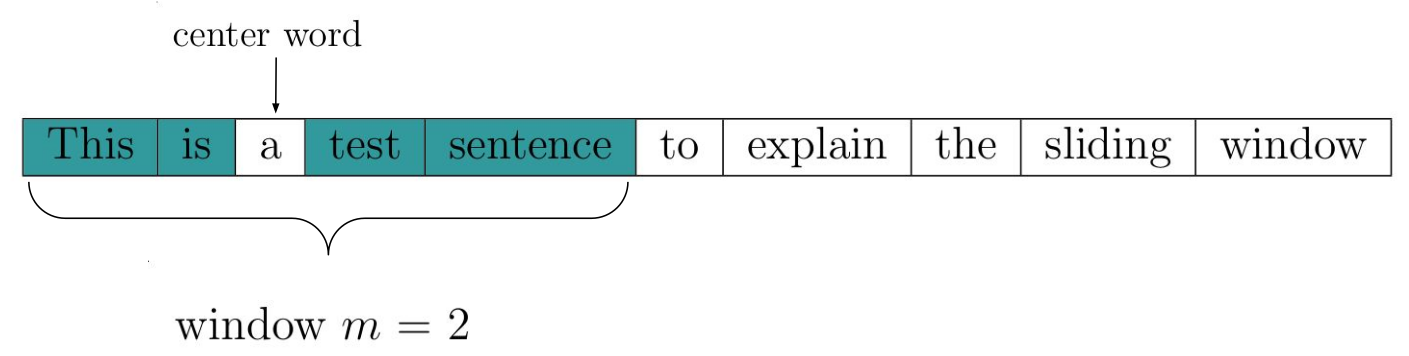
\includegraphics[scale=0.3]{images/window_ex}
\caption{Example of a center word and it's context words}
\label{fig:window_ex}
\end{figure}
%TODO think about example matrix
With these definitions the fake task can be defined: given a pair of center and context words, which will be our training samples, the goal of the network is to predict the probability of each word to appear in the context of the center word. One may ask how such a network is built. The network consists of two matrices, a projection and an output layer. Both of these matrices store word embeddings. The first one, the projection layer, will store the WE for one specific word in one specific row. It will have dimension $T\times d$, with $T$ being the size of our vocabulary and $d$ the dimension of our WE. The second layer, the output layer, will store one WE in each column. The idea behind these 2 layers is that the input layer will represent our words as center word and the output layer as context words. Since the task of the network being to predict the probability of each word appearing in the context of a given center word, the following probability should be maximized:\\
\begin{equation} \label{eq:basicSkip}
\prod_{t=1}^T \prod_{-m<j<m} p(w_{t+j}|w_t)
\end{equation}
Where T is the number of words in the corpus data, $w_t$ the $t^{th}$ word in the corpus data and $m$ is the context window. This means that the $m$ nearest words to $w$ are considered as context words.
Equation \ref{eq:basicSkip} can be transformed into sums by using log probabilities:
\begin{equation}
\sum _{t=1}^T \sum_{-m<j<m} log( p(w_{t+j}|w_t) )
\end{equation}
where the parameters are the same as in Equation \ref{eq:basicSkip}.

The basic Skip-Gram Model uses a classical Softmax to calculate the conditional probability $p(w_{t+j}|w_t)$:
\begin{equation} \label{eq:softmax}
p(w_{t+j}|w_t)= \frac{exp( \tilde{v}_{w_{t+j}}^Tv_{w_t})}{\sum_{w=1}^v exp(\tilde{v}_w^Tv_{ w_t})}
\end{equation}

Here $\tilde{v}_{w_t}$ and $ v_{w_t}$ are the vector representations, stored respectively in the projection Layer (first Matrix) and in the output layer (second Matrix). There is a problem with the classical softmax. As a matter of fact, it is unsuitable to compute the softmax. For the computation of $\sum_{w=1}^v exp(\tilde{v_w}^T w_t)$, the denominator in Equation \ref{eq:softmax}, one has to go over the whole corpus data. As very big data sets are needed to train the model, this is not a solution. Mikolov et al. \cite{mikolov2} proposed different solutions. The first solution is to use a Hierarchical softmax introduced by Morin and Bengio \cite{hsoftmax}. In this model, the probability distribution of the output nodes is saved in a binary tree which gives one a logarithmic computation time for each of these probabilities and makes it suitable to compute the softmax. Another possibility is the use of negative sampling which is discussed in the next subsection.

\subsection{Negative Sampling}
A second alternative solution to the use of a classical softmax is negative sampling. Negative Sampling is a simplification of Noise Contrastive Estimation (NCE) which was introduced by Gutmann and Hyv{\"a}rinen \cite{nce-original}, and first applied to NLP by Mnih and Teh \cite{mnih}. This subsection will shortly describe NCE and then how Mikolov et al. \cite{mikolov2} simplified it to create the technique called negative sampling. \\ The idea behind NCE is to distinguish data from noise. It does so by reducing the problem to a logistic regression task and does it by maximizing the log probability. The SGM is only interested in good word representation, hence the probability of the word is not meaningful as long as the quality of the word representations remains high. Mikolov et al. \cite{mikolov2} simplified NCE and called it Negative Sampling, which will be explained next.\\
The main goal of negative sampling is to only update the output nodes of certain words. This will obviously save an enormous amount of computation time. The idea is that given a pair $(c,w) \in D$, where $c$ is a word in the context window of $w$ we select $K$ random words $k_i$ from the corpus data $D$. We assume those words do not appear in the context of $w$. We denote the score that the $(c,w)$ wasn't drawn at random the following way: $p(y=1|c,w)$, and if $(k,w) $ is chosen at random this way: $p(y=0|k,w)$. Now we use logistic regression to update the weights of the $k$ selected context words and $c$. By doing so we will only have to update $k+1$ nodes.

Let's look at how we construct our objective function for a given word $w$ and one of its context words $c$:

\begin{align*}
p(c|w) &= p(y=1|c,w) + \prod_{k\in K} p(y=0|k,c)
\\&= p(y=1|c,w) + \prod_{k\in K} 1- p(y=1|k,c)
\\&= log((p(y=1|c,w)) + \sum_{k\in K} log(1- p(y=1|k,c))
\\&= log(\frac{1}{1+e^{-v_c \tilde{v_w }}}) + \sum_{k\in K} log(1-\frac{1}{1+e^{-v_c \tilde{v_k}}})
\\&= log(\frac{1}{1+e^{-v_c \tilde{v_w } }}) + \sum_{k\in K} log(\frac{1}{1+e^{v_c \tilde{v_k} }})
\\&= log(\sigma(v_c \tilde{v_w } ) + \sum_{k\in K} \sigma(log(-v_c \tilde{v_k} )) &&\text{where, $\sigma(x) = \frac{1}{1+e^{-x}}$}
\end{align*}\label{eq:obj_neg_samples}

Where $v_c$ and $\tilde{v_w }$, can be interpreted as before in Equation \ref{eq:softmax}. The goal is to maximize this objective function. Another way to look at this function, apart from logistic regression, and understand why it's working so well, is to assume that two vectors are similar if their dot product is high. Therefore, we maximize the dot product of similar words $(w,c)$ ($c$ appears in the context of $w$) and minimize it for dissimilar words $(w,k_i)$ (those were selected randomly).
We see that to compute our objective function we will only have to compute the sum over the number of negative samples $K$, which is very small in practice (2-20). To put things in perspective lets imagine our data set consists of 100000 words, we set $K=2$. Assume each output neuron has a weight vector $v$ with $|v| = 300$. In consequence, when updating our weights we would only update $0.2*10^{-2}$ of the 300 million weights in the output layer.

One question remains: how do we choose our random words? Mikolov et al. \cite{mikolov2} used the following unigram distribution:

\begin{equation} \label{eq:unigram}
P(w)=\frac{f(w)^{\frac{3}{4}}}{\sum_{t=0}^{T} f(w_t)^{\frac{3}{4}}}
\end{equation}
where $f(w)$ is the frequency of $w_t$. The value of $\frac{3}{4}$ is set empirically. Raising the unigram distribution to power of $\frac{3}{4}$ makes it less likely for a word to be drawn if it often appears in the dataset in comparison to the basic unigram distribution. See figure \ref{fig:frequency_ex} for an example.
\begin{figure}[ht]
\centering
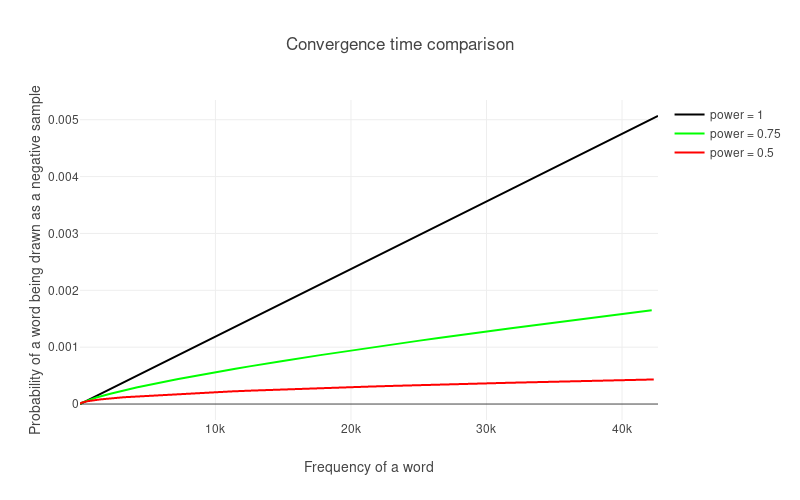
\includegraphics[scale=0.45]{images/frequency_ex}
\caption{Probabililty of a word, of the text8 dataset (sampled), to be chosen at random according to its frequency and the power to which the unigram distribution is raised}
\label{fig:frequency_ex}
\end{figure}
It's quite easily observable that this approach will outperform the classical softmax in computation time, as it only compute the sum over $K$ output nodes. Now the question arises if the accuracy is good enough but according to Mikolov et al. \cite{mikolov2} the negative sampling method "is an extremely simple training method that learns accurate representations". As a matter of fact, Mikolov et al. \cite{mikolov2} reported a 6\% accuracy improvement in comparison to a Hierarchical Softmax model. Therefore, it is a good solution to the problem raised by the classical softmax.
We now have enough background knowledge about the SGM to look at how it can be optimized. The next subsection introduces earlier approaches to optimize the SGM.

\section{Related Work}
Due to the popularity of the SGM, a lot of research went into optimizing it. This research can be divided into two categories, optimization of the throughput and the optimization of the algorithm's accuracy. The latter was achieved by allowing words to have multiple meanings, also called context-sensitive word embedings. For our work, the optimization of the throughput is of big interest while the semantic optimization is aimed at giving the reader a more holistic comprehension of the possible research directions.
This subsection will first give an overview of the optimization of the throughput and then present one paper that focused on context-sensitive word embeddings.

\subsection{Optimization of the throughput}

In the original model, the optimization is done with Stochastic Gradient Descent (SGD), which is a sequential algorithm. This process does not favor parallelization. To deal with this specific problem Mikolov et al.\cite{mikolov2} used a Hogwild tree proposed by Recht et al.\cite{hogwild}. The approach is to allow multiple threads to access a shared memory, in this case, the single model. In the original SGM, the threads are constructed as follows: at the beginning of training, the dataset is split into $N$ evenly sized chunks and each of these chunks will be processed by a one thread. The threads run parallel and have access to the shared memory. Therefore, overwriting errors are bound to happen. According to Recht et al.\cite{hogwild} the overwriting errors won't lead to a significant accuracy loss if the data is sparse enough. But in the case of NLP, the problem seems to be a bit more significant, and especially for word embedding, as many words share the same context words. There were several attempts at solving this issue, and we are going to cover a few of them in the following subsubsections.

\paragraph{Parallelization by the use of caching}
This idea was proposed by Vuurens et al. \cite{efficient}. The architecture used here is the basic skip gram model with a hierarchical softmax. The general idea is to cache the most frequently used nodes of the binary tree used to memorize the probability distribution and update them on the shared single model after a certain number of seen words (the paper used the number 10). The paper produced interesting results as they managed to decrease execution time by increasing the number of cores used for the calculation. This is very powerful because in the original implementation the execution time regressed after using more than 8 cores. It seems to indicate that too much overwriting was happening, as the number of concurrent threads surpasses a certain threshold. This can be seen in Figure \ref{fig:efficient}, where c31 is the model proposed by Vuurens et al.\cite{efficient}. The model did not suffer any accuracy loss in comparison to the original SGM model.
\begin{figure}[ht]
\centering
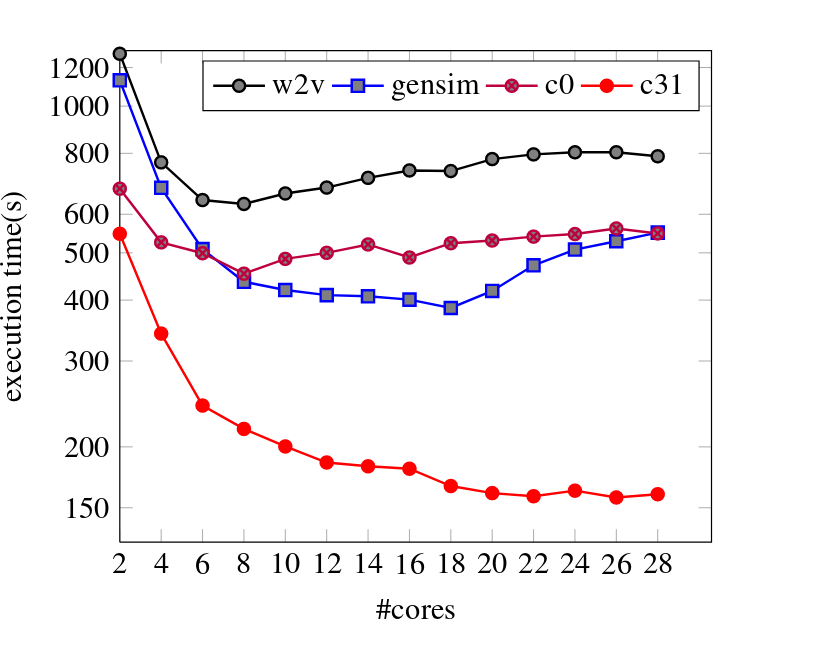
\includegraphics[scale=0.3]{images/cachingEfficiency.png}
\caption{Comparasion of the execution time in relation to the number of used cores \cite{efficient}}
\label{fig:efficient}
\end{figure}
This work proposes a very good way to parallelize the SGM, as in particular, it allows using more cores during the computation. As this approached focused on the Hierarchical softmax, in contrast to our work which used negative sampling, the next subsection covers optimizations of the Skip-Gram Model with negative sampling(SGNS).

\paragraph{Parallization in shared and Distributed Memory}
The first parallelized solution which was proposed by Ji et al. \cite{intel}, is to try to reduce the cost of our vector multiplication. The main idea in this paper is to convert the level 1-BLAS (Basic linear subprogram) vector to vector operations to a level 3-BLAS matrix multiplication operation, which are efficiently implemented into hardware and consequently faster. This is achieved, by using the same negative samples for each context word of a given word $w$. Instead of using for each context word a vector to vector multiplication we can transform this into a matrix multiplication, under the assumption that we will not lose accuracy by sharing the same negative samples. The matrix multiplication can be represented in the following way.
\[
\begin{bmatrix}
w \\
w_{n_1} \\
\vdots \\
w_{n_k}\\
\end{bmatrix}
*
\begin{bmatrix}
w_{c_1}\\
\vdots\\
w_{c_{2m}}\\
\end{bmatrix}
\]

where $w$ is our given word, $w_{n_1}...w_{n_k}$ are the shared negative samples, with $k \in [5,20]$, and $w_{c_1}...w_{c_2m}$ are the words inside of the context window $m$ of $w$, with $m \in [10,20]$, also called a batch of input context words. After each batch the model updates the weights of the used vectors.
This model achieves a 3.6 fold increase in throughput, by only losing 1\% of accuracy. An aspect that is not as useful to us is that the experiments were done on CPU, as modern GPU's are often used in many machine learning libraries, as with CUDA for example, there still need work to be done to optimize it with GPU's. This was done by Seulki and Youngmin \cite{gpu}, which is described in the next subsection.

\paragraph{Accelleration of word2vec by Using GPU's}
Seulki and Youngmin \cite{gpu} focused on getting a better throughput on the SGM when using GPU's. As the SGM is a sequential algorithm, is is not easy to parallelize it, especially if one wants to parallelize the training of individual training samples. As the algorithm goes sequentially over a sentence, the samples next to each other, in order of execution, will almost every time have the same input word. Consequently, it's very hard to parallelize at this level. To solve this problem, Seulki and Youngmin \cite{gpu} proposed the idea to parallelize the update of each dimension of the word embedding, since those are completely independent of each other. They achieved this by mapping each dimension to a CUDA thread while mapping each sentence to a CUDA block. As each CUDA block runs independently, the training of the sentences is parallelized, and the fact that sentences have different length is of no problem. If the execution time of the GPU kernel is greater than time used to read the sentences, it could be a smart choice to use multiple GPU's. According to Seulki and Youngmin \cite{gpu}, if multiple GPU's are used, there is a need for synchronizing the model, which will hinder run time performance. They achieved their best results with 2 concurrent GPU'S. The accomplished results were very good as they managed a 20x speedup compared to a single threaded CPU execution, which is a 3x increase in comparison to the original C code from Mikolov et al. \cite{mikolov2}, with no loss in accuracy. The problem with this and all the above optimization is that the code is not easily available. Therefore, we need an optimized implementation of the SGM that is easily available. This is provided by Gensim \cite{gensim}, which will be outlined in the next subsection.
%%%%%%%%%%%
\paragraph{Gensim}\label{ssec:gensim}
Gensim \cite{gensim} is a pure Python library that holds a state of the art implementation of the SGM. Gensim is written in Cython, which first allowed Gensim to have the same runtime as the original C code. Furthermore, it made use of BLAS's and precomputed sigmoid tables, while also trying to parallelize the training of different sentences. This finally yielded in a 4x speedup in run time. Gensim is an important tool as it allows us, as a python library, to compare our data rather easily. It was also used in related work \cite{intel} and is therefore of value, as it allows to us compare our work in a simpler way. This concludes our overview of the optimizations of the throughput of the SGM. In the next subsection, we give a quick outlook of what has been done in the field of context-sensitive word embeddings.

\subsubsection{Context sensitive word embedding}
A word has different meanings dependent on its context. This is a problem that is not addressed by the SGM. Some new models, that have taken this issue into consideration, were proposed. A lot of work has been done in this direction, Liu et al.\cite{topicalWE} and Bartunov et al.\cite{breaking} for example, but the one reporting the best results is Liu et al. \cite{contextWithTensor}. The concept of this approach is to change the way we compute the objective function and variables we use in our conditional probability. The idea is to look if a word given a certain context word matches to a topic. \textit{Bank} would match to \textit{finance} given the context word \textit{money}. \textit{Bank} would also match to \textit{nature} if \textit{river} was the given context word. But \textit{Bank} would not match to \textit{nature} with the context word \textit{money}. Now one could ask how to achieve such a context sensitive word embedding? First, we have to introduce new variables, therefore let's look at the objective function used:
\begin{equation}
J(\Omega) = \sum_{(w,t,c)\in D} \sum_{(w,\tilde{t},\tilde{c} \in{\tilde{D}})} max(0,1- g(w,t,c) + g(w,\tilde{t},\tilde{c})) \lambda||\Omega||_{2}^2
\end{equation}

This approach uses the same negative sample technique as described in the previous subsections, $D$ is the corpus data and $\tilde{D}$ is the set of negative samples and $\lambda$is the hyper parameter used for the standard $L_2$ standardization. What is interesting here is the function $g(w,c,t)$, where $w$ is a word, $c$ the context word, and $t$ the context in which the word appears. $g$ is defined as follows:
\begin{equation}
g(w,c,t) = u^T \sigma(w^TM^{[1:k]}t+V_c^T(w \oplus t) + b_c)
\end{equation}
where, $u, V_c, b_c$ are standard parameters for a neural network. $\oplus$ is the vector concatenation. The most important parameter is $M^{[1:k]}$, which is a tensor layer, the tensor layer is used because of its ability to model multiple interactions in the data, as this will be useful for multiple contexts. They used SGD for the optimization of this objective function. They achieved interesting results as shown in \ref{fig:multipleContext}.\\
\begin{figure}[ht]
\centering
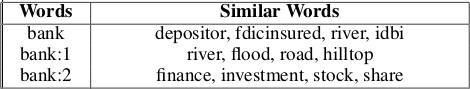
\includegraphics[scale=0.7]{images/multipleContext.png}
\caption{"Nearest neighbor words model and Skip-
Gram. The first line in each block is the results of Skip-Gram;
and the rest lines are the results of our model" \cite{contextWithTensor}}
\label{fig:multipleContext}
\end{figure}

This will conclude our overview of the related work. We will now give the reader an outline of the different Gradient Descent Optimizer used in our experiments.

\section{Results}\label{chap:results}

%Describe the experimental setup, the used datasets/parameters and the experimental results achieved

This subsection gives an overview of the used datasets, the used metric to evaluate our models, the configuration of our model and finally, the experimental results achieved.

\subsection{Dataset}\label{sec:dataset}
In this implementation we only used the text8 \footnote{http://mattmahoney.net/dc/enwik8.zip} dataset. We chose this dataset for two reasons. First of all, it's a very small dataset, that allowed us to do a lot of computations. Secondly, this dataset was used in related work \cite{intel} hence giving us a very good benchmark. The text8 dataset consists of 1702 lines of 1000 words, with a vocabulary of roughly 63000 words. Conveniently, there is no punctuation in the dataset. Therefore, we had to choose between building arbitrary sentences and keeping the dataset as it is. We chose the first option because it gives us a faster computation time, and did not show any significant loss in quality empirically, as shown in Table \ref{table:with_20}. We chose a length of sentences of 20. Furthermore, we applied a technique called subsampling to reduce the data set size, which is explained in the following subsection.

\begin{table}[]
\centering
\begin{tabular}{|l|l|l|l|l|}
\hline
Length of Sentences & 10 & 20 & 40 & 1 Document \\ \hline
Training Time for one batch &8min & 10min & 11min & 18min \\ \hline
Convergence Time &4 epochs & 3 epochs & 3 epochs & 3 epochs \\ \hline
Word Similarity& 0.65 & 0.66 & 0.66 & 0.66 \\ \hline
\end{tabular}
\caption{Training and Convergence time according to choice of the length of sentences in text8 dataset}
\label{table:with_20}
\end{table}

\subsubsection{Subsampling}
Subsampling is a technique introduced by Mikolov et al. \cite{mikolov} to reduce the dataset size while at the same time increasing the quality of the dataset, i.e getting better word embeddings with it. The idea behind subsampling is the removal of very frequent words such as: "the, as, it, of". These words do not give an intrinsic value to the words that appear in its context. Therefore, the goal of subsampling is to delete such words from the dataset. This will decrease the computation time, as it will reduce the number of training samples, and should, in theory, increase the accuracy of the model. The increase in accuracy can also be explained by the fact that words that would not have appeared in the context of each other, may now do because words between have been deleted.
To choose which word to delete, Mikolov et al. \cite{mikolov2} chose the following equation to compute the deletion of a word $w$ in the data set:
\begin{equation} \label{eq:sampling}
P(w) = 1- \sqrt{{\frac{t}{f(w)}}}
\end{equation}

where $f(w)$ is the frequency of w, and $t$ is a threshold set empirically. As Equation \ref{eq:sampling} is a probability, subsampling is not a deterministic procedure, words that may have been deleted with a threshold of $10^-2$ may stay in the dataset with a lower threshold, as shown in Table \ref{table:treshold_examples}. Mikolov et al. recommend a value between $0$ and $10^{-5}$, depending on the size of the dataset. We experimented with different values and $10^{-4}$ seemed the most suited. We did this by looking at a random set of sentences and judging the results manually. An example of the first sentence with different sampling thresholds can be found in Table \ref{table:treshold_examples}. The table shows the first 20 words of our dataset, without the words that were subsampled according to a threshold sample. Stats about subsampling can be found in Table \ref{table:treshold}.
\begin{table}[h]
\centering
\begin{tabular}{|l|l|l|l|l|l|}
\hline
Sampling Treshhold & 0 & $ 10^{-1}$&$ 10^{-2}$& $10^{-3} $ &$10^{-4} $ \\ \hline
Number of words in Dataset & 16 mio & 15mio & 11 mio & 8mio & 4 mio \\ \hline
\end{tabular}
\caption{Size of the preprocessed text8 dataset according to sampling treshold}
\label{table:treshold}
\end{table}

\begin{table}[]
\begin{tabular}{|l|l|}
\hline
Sampling Treshold & First sentence of Dataset \\ \hline
$10^{-1}$ & \begin{tabular}[c]{@{}l@{}}Anarchism originated as a term of abuse first used against early\\ working class radicals including the diggers of the english\end{tabular} \\ \hline
$10^{-2}$ & \begin{tabular}[c]{@{}l@{}}Anarchism originated as a term of abuse first used against early \\ working class radicals including diggers of english\end{tabular} \\ \hline
$10^{-3}$ & \begin{tabular}[c]{@{}l@{}}Anarchism originated a term abuse first used against early \\ working class radicals including diggers the english\end{tabular} \\ \hline
$10^{-4}$ & \begin{tabular}[c]{@{}l@{}}Anarchism originated abuse used against working class radicals\\ diggers english\end{tabular} \\ \hline
$10^{-5}$ & against radicals diggers \\ \hline
\end{tabular}
\caption{Example of a sentence with different sampling tresholds}\label{table:treshold_examples}
\end{table}

\subsubsection{Min count}
We also deleted every word that did not appear more than 5 times in our dataset. We got this technique from Gensim \cite{gensim}, that introduced this parameter into their training. This is a good technique because of three reasons: First certain words of our data sets do not appear in a common lexicon (twigleg, melqu), or come from a foreign language (Volksvereinigung), or are names and acronyms. Secondly, each document often has spelling mistakes, those (as long as the same spelling mistake does not appear too often, what should be avoided in practice) would be deleted by sampling too, as the words do not have any meaning. Lastly, a word that only appears one time in our dataset will be very dependent on its original initialization. This is the case because it will only be updated with its context pairs once, which is only a dozen of times in practice and then won't be updated anymore. For all the above reasons, we applied this technique. Similar to subsampling, it should in theory improve the quality of the word embeddings and will decrease the computation time.

\subsection{Evaluating word embedings}
Evaluating word embedding is not an easy task, such as evaluating the accuracy of a common classifier. We cannot split our data set into train and test set. As the task that the network is learning is of no interest to us. Therefore, we need to verify that our embedding is of quality with other techniques. To define quality we first need to define a measure of similarity between two vectors. This requires knowledge of the Cosine distance, which is introduced in the following subsection.
\subsubsection{Cosine distance}
The cosine similarity, this is not the cosine distance, of vectors $v$ and $w$ is the cosine of the angle between the two vectors It can be calculated by taking the dot product of $v$ and $w$ and dividing it by the magnitude of $v$ and $w$ multiplied with each other. We get:
\begin{equation}
cos\_sim(v,w) = \frac{v \cdot w}{|v| |w|}
\end{equation}
The cosine of 0\textdegree ~is 1, it's 0 for two vectors that are orthogonal to each other and vectors that point in the opposite direction will have a cosine of their angle of -1. This is not a good distance measure as -1 is smaller than 0, and therefore two vectors pointing away from each other would be closer than two orthogonal vectors, but by subtracting 1 from the cosine of the angle we can create a good distance measure between the two vectors. This distance does not take into account any order of magnitude. Hence, for our tasks, two vectors will be considered equal if they are of different magnitude but point in the same direction.
Apart from measuring the quality of word embedding well, this technique has another advantage. By normalizing the vectors the calculation of the cosine angle becomes the dot product of the two vectors. Which can be computed very fast on modern GPU's.
Knowing that we have a measure to compute the similarity of two vectors let us introduce a way to rate the quality of our embeddings.

\subsubsection{Word similarity and wordsim353}
To measure the quality of our word embedding we will need a dataset to compare our results too. We chose wordsim353\footnote{http://www.cs.technion.ac.il/~gabr/resources/data/wordsim353/wordsim353.zip} for this task, as it's the most used in the related literature. The data set consists of 353 pairs of words rated by humans on their similarity. The similarity score is in the range of 1 and 10, with 10 being the best score. An example for two of such pairs can be found in Figure \ref{fig:ws353_ex}. We will rank our embeddings on the Pearson correlation coefficient between the cosine distance and the scores attributed by humans, as this is a common procedure.

\begin{table}[]
\centering
\begin{tabular}{|l|l|l|}
\hline
Word1 & Word2 & Score \\ \hline
\textquote{FBI} & \textquote{Investigation} & \textquote{8.31} \\ \hline
\textquote{Mars} & \textquote{scientist} & \textquote{5.63} \\ \hline
\end{tabular}
\caption{Example of pairs and their rating in wordsim353}
\label{fig:ws353_ex}
\end{table}

\subsection{Configuration of the network}
The skip gram model has a lot of possible parameters, that can be tuned. We experimented with different models and finally decided for one that we tried to optimize. This subsection will give a short overview of each parameter, where we will explain the process in which we chose the value of the given parameter. The explanation of the parameters will be structured as follows:
\texttt{Parameter} - Description and tuning - \textit{Value}
\begin{itemize}
\item \texttt{Negative Samples:} Here we have to find a trade-off between, setting the parameter too high which will result in increased accuracy but a longer computation time. For smaller data sets a higher number of negative samples is often needed. In their original paper Mikolov et al. \cite{mikolov2} recommend a value of 5-20. We tested a few values in the range of 5 to 15, as 10 yielded state of the art results we chose this value. - \textit{10}
\item \texttt{Context Window:} The bigger the window the more training examples the network will have, but if the window is too big the semantic meaning of the window will be erased. Mikolov et al. \cite{mikolov} proposed a setting between 2-10, as all our sentences are of size 20 we chose 5. - \textit{5}
\item\texttt{ Dimension of the embedding}: Here the choice is less obvious, as the dimension needs to be high enough to capture the meaning, but cannot be too high as this leads to a decrease in performance as shown by Yin and Shen \cite{dimension_size}. We, therefore, used Gensim to find the best embedding possible. - \textit{100}
\item \texttt{Batch size}: As described in subsection \ref{ssec:b_SGM}, there is a tradeoff to find between quality and training time. We first used a batch size of 5000, but then decide after non conclusive results (see \ref{ssec:bs_lf}) that 2000 would be better - \textit{2000}
\item \texttt{Alpha}: learning rate, this hyperparameter was tuned in every optimizer therefore only the range will be indicated - \textit{(1e-5,1)}
\end{itemize}

\iffalse
\begin{table}[h]
\centering
\begin{tabular}{|l|l|}
\hline
Embedding Size & Word Similarity on Gensim \\ \hline
50 & 0.65 \\ \hline
100 & 0.67 \\ \hline
200 & 0.65 \\ \hline
300 & 0.63 \\ \hline
\end{tabular}
\caption{Word similarity in relation to the size of the embedding}
\label{table:gensim_emb_size}
\end{table}
\fi
\subsection{Input Shuffling}
We used input shuffling as a technique to optimize the skip gram model. We will first describe input shuffling in a general way and then explain why we suppose that input shuffling could work well on the skip gram model. \\
Let $X = {x_1...x_n}$ be our input data set. Input Shuffling describes the process of taking a random permutation of the dataset as input at each epoch.
The idea behind this technique is to present our optimizer with different loss surfaces so that it's able to find the best optimum. Therefore, it's easier for the neural network to escape a local minimum. As for example if a network had converged to a local minimum after one epoch it could not escape it as all the parameters are the same. But if we change the shape of the loss function, by input shuffling, then there would be a greater probability for the network to escape the local minimum.
\\
There are two reasons why we think that input shuffling is particularly well suited for the skip gram model. The first one has to do with the fact that when we read our words sequentially that words that only appear very early will not benefit from the context words being already updated from others. The second idea is that we used the special batch technique described in Section \ref{ssec:b_SGM}. When using this technique and not using shuffling we will always have words that appear next to each other in a batch and will, therefore, update the same words at the same time. We, therefore, lose some quality. But if we would use input shuffling instead, then the words in one batch would likely not be similar and therefore only taking the average of a small part of pairs with the same words will be less likely.

\subsection{Convergence time}
To optimize convergence time we have to define it first. Therefore, we used the already available implementation of Gensim \cite{gensim}. Gensim is an open source software that proposes an implementation of the SGNS in Python. It is also written in Cython, therefore it has a fast computation time, but can be used inside a python implementation. Together with the knowledge from Ji et al.\cite{intel} that a score of $0.66$ in the task of word similarity, with the text8 dataset, is the state of the art, we tested Gensim (more on this process in subsection \ref{chap:discussion} and found out that it took 4 epochs to converge. Therefore, we defined the following criteria for convergence: \\
$\rho - \rho_{prev} < 0.009 \vee \rho = 0.66$ \\
where $\rho$ is the Pearson coefficient on the wordsim353 task.
We also stopped computation, if it took more then 20 epochs to converge.

\subsection{Results by optimizer}
We ran multiple experiments for each optimizer. This subsection will only give an overview of the achieved results. Each subsection will give an explanation over the achieved result with a specific optimizer.

\subsubsection{SGD}
The first challenge for each optimizer was to find a correct learning rate. As SGD is the optimizer used in Gensim \cite{gensim} we first tried the same learning rate as Gensim \cite{gensim} and then performed a random search to find a better one. As expected a bell curve shape resulted, a learning rate that is too high leads to diversion and a learning rate that is too low leads to a training time that is too slow. The best value that we found for the learning rate is $0.0075$. With this setting SGD converged in 11 epochs. The second experiment was to add input shuffling.
As seen in Figure \ref{fig:results_sgd}, for almost every learning rate the convergence time decreased. Our model, with the best setting, now converges in only 7 epochs. Another interesting fact to point out from Figure \ref{fig:results_sgd} is that with input shuffling we achieved better results with higher learning rates. As for learning rates of $0.01$ and $0.025$ we did converge in 11 epochs with input shuffling but did not converge in 20 epochs without it.

\begin{figure}[h]
\centering
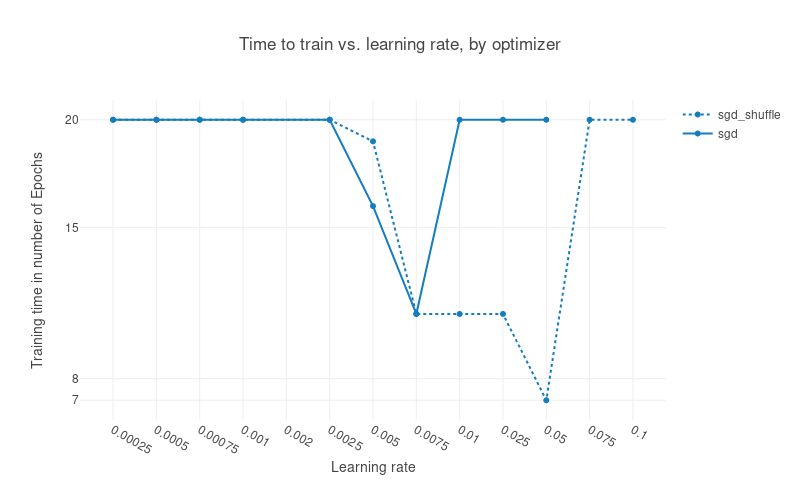
\includegraphics[scale=0.45]{images/results_sgd_shuffle}
\caption{Training time Stochastic Gradient Descent with input Shuffling}
\label{fig:results_sgd}
\end{figure}
\subsubsection{Momentum and Nesterov}
Momentum and NAG \cite{nag} both have an additional hyperparameter $\gamma$, that, as described in Section \ref{optimizers}, defines the percentage of the previous gradient that will be added to the current gradients. We set $\gamma = 0.9$ as this is the typical value and did not alter it during our experiments. Momentum and Nesterov alone respectively only slightly decrease or increase the convergence time. Momentum optimally converges in 9 epochs and Nesterov in 13. If we combine these optimizers with input shuffling, interestingly the same phenomena as with plain SGD appear. The convergence time gets better, 8 epochs for Momentum and 3 epochs for NAG. The phenomena that a higher learning rat yields better results also happens with both of the optimizers. As Momentum does not converge in 20 epochs with a learning rate of 0.002 but does in 8 with input shuffling.
\begin{figure}[h]
\centering
\begin{minipage}{.5\textwidth}
\centering
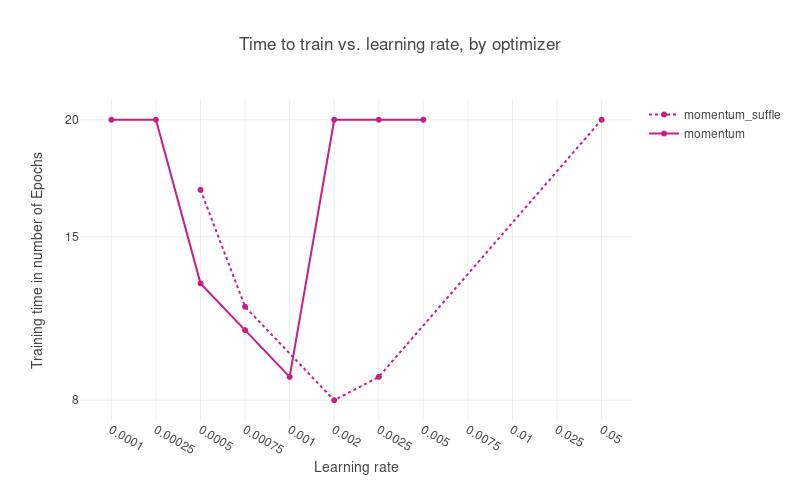
\includegraphics[scale=0.3]{images/results_mom_shuffle}
\caption{Training time Momentum with input Shuffling}
\label{fig:results_mom}
\label{fig:test1}
\end{minipage}%
\begin{minipage}{.5\textwidth}
\centering
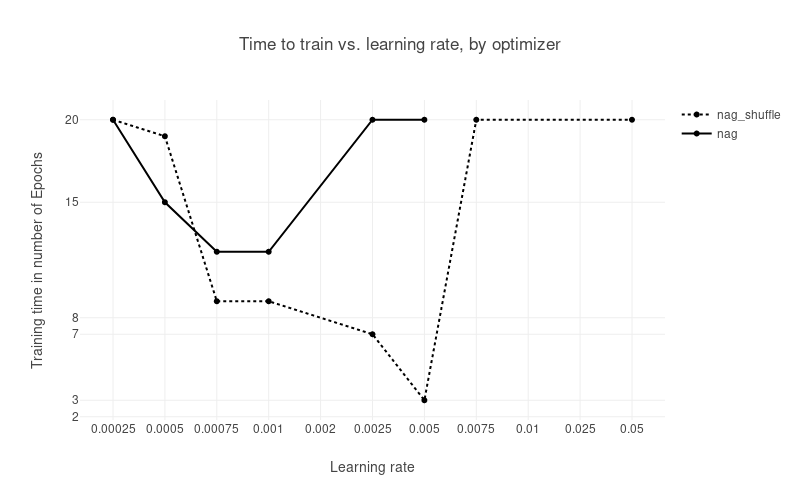
\includegraphics[scale=0.3]{images/results_nag_shuffle}
\caption{Training time Nesterov with input Shuffling}
\label{fig:results_nag}
\end{minipage}
\end{figure}
\subsubsection{Adagrad}
Adagrad \cite{adagrad} is a very interesting tool for learning word embeddings as it decreases the learning rate for very frequent occurring features, and vice versa (this is explained in detail in Section \ref{ssec:adagrad}). Because words that appear very frequently often do not have a semantic gain that is as important as words that appear less frequently to their context words, it's good to have a lower learning rate. So, in theory, Adagrad is particularly well suited for our task. This was confirmed empirically as our model converged in 4 epochs. When combined with shuffling Adagrad only took 3 epochs to converge. This shows the tendency of the skip gram model to converge faster with input shuffling and the big impact of having different learning rate for each feature.
Here it's interesting to notice that a higher learning rate combined with input shuffling did not yield better results than without shuffling. Both of our best results happened with a learning rate of $0.1$, as shown in Figure \ref{fig:results_adagrad_shuffle}.
\begin{figure}[h]
\centering
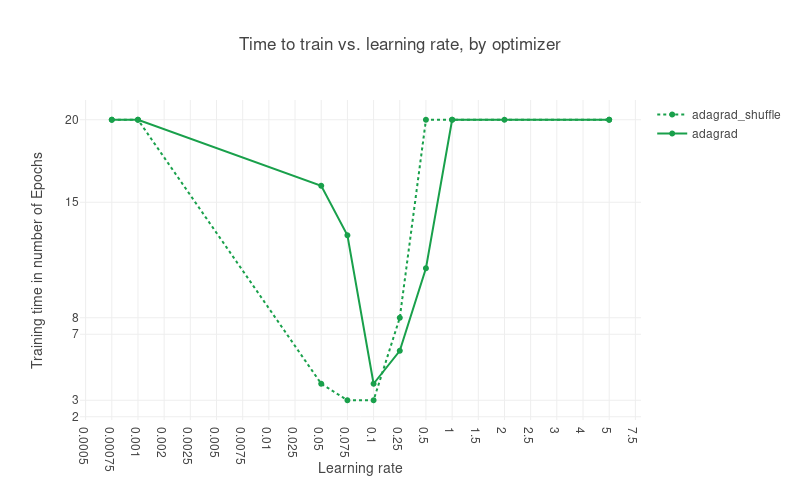
\includegraphics[scale=0.45]{images/results_adagrad_shuffle}
\caption{Training time Adagrad with input Shuffling}
\label{fig:results_adagrad_shuffle}
\end{figure}
\subsubsection{Adadelta}
In theory Adadelta \cite{adadelta} should outperform Adagrad as it's an extension of the former. Because it didn't have any learning rate to tune, we only did 2 experiments, with and without input shuffling. We are aware of the fact that there are additional hyperparameters but did, for simplicity reason, and because their effect is not as high as the learning rate in other optimizers, decide not to tune it. We left it to its default value $\rho = 0.9$. This parameter defines the percentage taken when calculating the exponentially decaying average of past gradients, as explained in \ref{ssec:adadelta} Adadelta did not manage to achieve a word similarity of 0.66. It only converged to a similarity of 0.59. It did this in 20 epochs without input shuffling and in 3 with input shuffling, as can be seen in Table \ref{table:results_adadelta}
\begin{table}[h]
\centering
\begin{tabular}{|l|l|l|}
\hline
Adadelta Model & Convergence Time & Word similarity \\ \hline
Without Shuffling & 20 & 0.59 \\ \hline
With Shuffling & 3 & 0.59 \\ \hline
\end{tabular}
\caption{Convergence Time and Quality with Adadelta}
\label{table:results_adadelta}
\end{table}


\subsubsection{Adam}
Adam is the most advanced of all the optimizers used in our experiments and did yield the best results as seen in Figure \ref{fig:results_adam_shuffle}. Adam converged in 3 epochs without shuffling and 2 with. This is the best result that we got with any optimizer.  It's also interesting to note that as same as with Adagrad it did not react to input shuffling the same way as SGD did. In fact, it worked in the opposite direction, as we achieved our best result with input shuffling while having a lower learning rate $0.001$ then we used to achieve the best result without input shuffling $0.05$.
\begin{figure}[h]
    \centering
            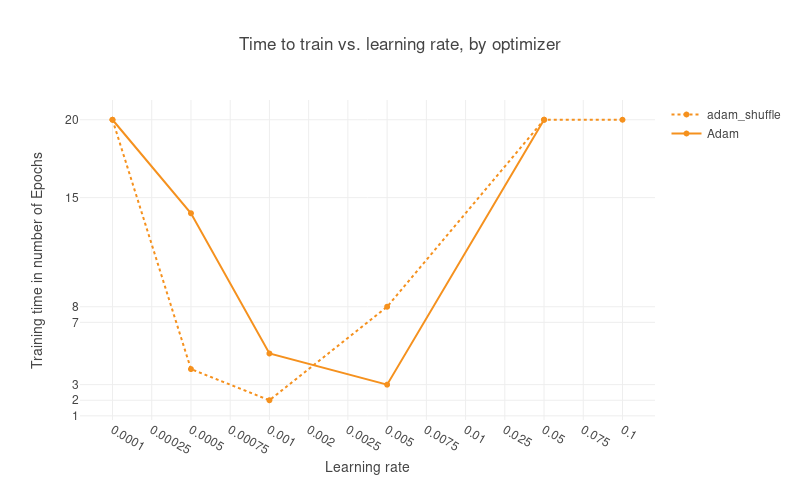
\includegraphics[scale=0.45]{images/results_adam_shuffle} 
    \caption{Training time Adam with input Shuffling}
    \label{fig:results_adam_shuffle}
\end{figure}

\section{Discussion}\label{chap:discussion}

%Discuss the results. What is the outcome of your experimetns?
This subsection shortly discusses the empirical results and then extensively compares the findings of this work to the existing literature while trying to explain some differences. It is followed by a subsection describing the limitations and possible extensions of this work. This subsection is concluded by the problems we encountered during the implementation so others can avoid them in the future.

\subsection{Our work}
This subsection discusses our findings, first we will analyze how input shuffling could influence the learning rate and conclude with the discussion of unexpected results.

\subsubsection{Shuffling and learning rate with SGD}
When the model used SGD as an optimizer it was able to use higher learning rates when input shuffling was used, as shown in figures \ref{fig:results_sgd}, \ref{fig:results_mom} and \ref{fig:results_nag} Therefore arises the questions why these phenomena happen, especially as it did not happen with advanced optimizers. One possibility is the use of the batched version of the SGNS. In consequence, when the input is not shuffled the same word will often appear in one batch, hence the optimizer is presented with an average value of the gradient, which can be imprecise. This is counter-attacked by advanced optimizers as they have adaptive learning rates, i.e a frequent appearing feature will have a low learning rate.

\subsubsection{Large differences with NAG and SGD when using shuffling}
SGD and NAG both have very different values when using shuffling in comparison to unshuffled input, as shown in figures \ref{fig:results_sgd} and \ref{fig:results_nag}, plain SGD. We do not only attribute those results to input shuffling but partially also to a good random initialization guess. Due to a lack of time these results were not replicate more than once.

\subsection{Comparison to Gensim}
This subsection will compare our finding extensively to Gensim \cite{gensim}. As explained in Section \ref{ssec:gensim}, Gensim is optimized to have a very high throughput, this made it possible to achieve a lot of computations. Furthermore, Gensim provides access to the loss and the resulting word embeddings, which facilitated the comparison process.

\iffalse
As Mikolov et al. published the original paper which introduced the SGNS, it is, of course, relevant to compare ourselves to their work. The first important thing to take under account is that Mikolov et al. only trained their model on a very large google news dataset incorporating more than 3 billion words. This makes the comparison of our work more difficult. But we will make some assumptions, as they could be of value if true.
In their original paper, Mikolov et al. reported results from computations that took 1 and 3 epochs. We accord these good results, which clearly outperformed our SGD model and Gensim, to the very large dataset and furthermore, as a matter of fact, their results are better with 3 than with 1 epoch. We do not have any information about the convergence time or criterion. Hence it would be interesting to use their dataset for comparison. \\
One thing we can compare is the quality of our word embeddings. Mikolov et al. did not report any results on their model with the text8 dataset, but they, therefore, published their code. Which was then used by Ji et al \cite{intel} and they tested the model on the text8 dataset. They reported a word similarity of 0.63 on the word similarity task. This is obviously outperformed by all our models. We did not find any explanation on why those results differ as much. \\
The final assumption is that an advanced optimizer could maybe outperform SGD in terms of quality on a large data set. This will be discussed in further work.

\fi

\subsubsection{Configuration of Gensim}
The training with Gensim has a lot of possible parameters an extended list can be found in the appendix. This subsection will only describe the parameters we changed from the default setting. The description of each parameter has the following form: \\
\texttt{name} (type) -- \textit{Description} -- Value\\
Parameters:
\begin{itemize}
\item \texttt{sentences} (iterable of iterables) -- \textit{Dataset} -- text8 document splitted into sentences of 20 words
\item \texttt{size}(int) – \textit{Dimensionality of the word vectors } -- 100
\item \texttt{window} (int) --\textit {Maximum distance between the current and predicted word within a sentence }-- 5
\item \texttt{min\_count }(int) --\textit{ Ignores all words with total frequency lower than this }-- 5
\item \texttt{workers} (int) -- \textit{ Number of threads used to train the model} -- 4
\item \texttt{sg} ({0, 1}) --\textit{ Training algorithm: 1 for skip--gram}--1
\item \texttt{negative} (int) --\textit{Number of negative samples}-- 10
\item \texttt{ ns\_exponent} (float) --\textit{ Exponent in the unigram distribution, when choosing random samples, as shown in Equation \ref{eq:unigram} }-- 0.75
\item \texttt{alpha} (float) --\textit{ The initial learning rate. }-- 0.025
\item \texttt{min\_alpha} (float) --\textit{ Learning rate will linearly drop to min\_alpha as training progresses }--0.0001
\item \texttt{sample} (float) --\textit{ Treshold for subsampling as described in Equation \ref{eq:sampling}} -- 1e--4
\item \texttt{iter} (int) --\textit{ Number of iterations (epochs) over the corpus. }-- 10
\
\item \texttt{compute\_loss} (bool) --\textit{If True, loss is stored at the end of each batch}-- True
\item \texttt{callbacks} (iterable of CallbackAny2Vec) --\textit{ Set of functions executed in order to follow the loss and the progress of the model in word similarity }-- see Appendix
\end{itemize}

\subsubsection{Gensim vs. SGD}
As stated earlier, we are not going to compare this work to Gensim in run time. Gensim is heavily optimized and written in cython\footnote{https://rare-technologies.com/word2vec-in-python-part-two-optimizing/}, which is 23x faster than plain Numpy. Since we used PyTorch the difference is not that big, but still remains. As shown in Figure \ref{fig:gensim_vs_adam} the convergence time was not the same between our implementation and Gensim. There are different possible reasons why this could be the case:\\ First, our batched approach could hinder performance in terms of convergence since our loss function is not exactly the same. When a word appears more than once in our batch, the gradient will be an average over the gradients of each pair alone, as it is done by Gensim.\\ Secondly, a difference to our implementation is the fact that Gensim checks whether negative samples are not equal to the context word. If that is the case Gensim selects a new random sample. Therefore, the learning of the input and output context is optimized. \\Finally, another possibility is the decay of the learning rate used by Gensim. In fact, decaying the learning rate has been proven in a lot of work to decrease the convergence time. Gensim linearly decreases the learning rate, as we did not use this technique, the decay of the learning rate could help explain the noted differences. \\ The first hypothesis, the fact that we used a batched approach, may be confirmed by the fact that when combined with input shuffling SGD does perform closer to Gensim, going from 11 to 7 epochs to converge, as input shuffling reduces the number of co-occurrence of the same word in a batch.
Now the question arises if the 3 epochs, that Gensim is better, can be explained by the selection of better negative samples and the learning rate decay?

\subsubsection{Gensim vs. Adam}
The Adam optimizer did outperform the Gensim application in quality of word embeddings (only slightly: 0.01 correlation coefficient better) and convergence time. Adam converged in 2 epochs while Gensim in 4. To confirm the achieved results we ran each computation 40 times. The results can be seen in Figure \ref{fig:gensim_vs_adam}.

\begin{figure}[h]
\centering
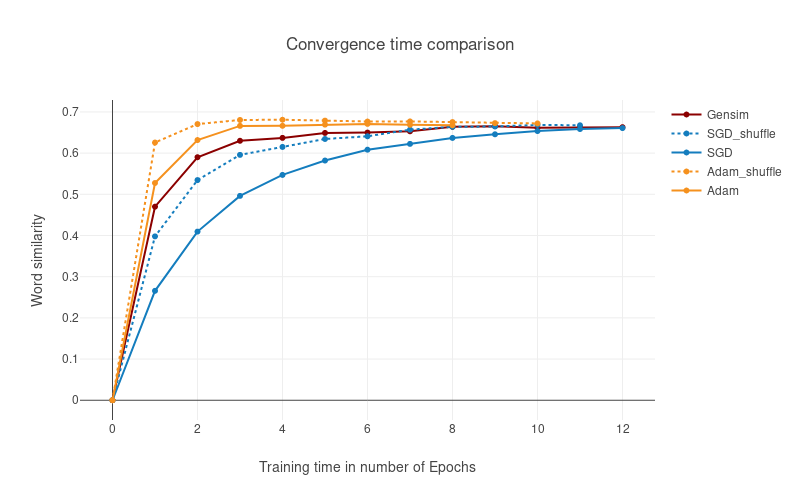
\includegraphics[scale=0.45]{images/gensim_vs_adam}
\caption{Convergence time of SGD and Adam compared to Gensim}
\label{fig:gensim_vs_adam}
\end{figure}\subsection{Challenges faced}
During our implementation we did encounter some problems, this subsection has the purpose of preventing the scientific community from making the same mistakes.
\subsubsection{Using the wrong embeddings}
To start with, we did not choose the same initialization value as Gensim in our word embeddings. We initialized the projection layer with a normal distribution between (-1,1), as opposed to Gensim which initializes all the weights to 0. The reason for this, is that at the beginning of our experiments we did not achieve good results with the same initialization as Gensim. Retrospectively we accord this to a learning rate that was too low. After a few simulations, we saw that we did not perform as good as Gensim. And as we changed the initialization of the projection layer back to 0, and already had adjusted the learning rate, we achieved good results. Therefore, this is a recommendation to future work to not set the initialization to (-1,1).

\subsubsection{Batch size and loss function adjustements}\label{ssec:bs_lf}
During our experiments, we faced a moment where we needed to us a very high learning rate (50) to achieve good results. As this is the complete opposite of what is standard we made a few changes to remedy the problem.\\
First, we needed to find a good batch size. During the above-explained raise of the learning rate, we used a batch size of 5000. We then decided to take a batch size of 2000.\\
Secondly, at the same time, we did experiment with different loss functions. As our batched model does not have exactly the same loss function as introduced by Mikolov et al. \cite{mikolov}, we needed to find one that suited our goals the best. At the beginning of our experiment, we took the average of all the scores stored in our final matrix, as explained in \ref{ssec:b_SGM}. But then chose to take the sum as the training did not seem optimal.\\
With these two changes, we did increase convergence time and word similarity, while at the same time having a usual learning rate. \\
Know the question arises why this happened? Is this because of the shape of the loss function better suits our advanced optimizers? Or because the loss function is closer to its original form? Our hypothesis looks the following way:
When taking the average, our loss function is represented as follows:
\begin{equation}
\frac{-1}{b }* \sum_{x\in X} loss(x)
\end{equation}
where $X$ is our batch and $b = |X|$.
When taking the partial derivative of each parameter, the constant $ \frac{-1}{b }$ will remain the same. Therefore, it's the same as taking the sum as the loss function and multiplying each gradient with $\frac{-1}{b }$. As our batch size was really high, i.e 2000 and 5000, this could highly influence the learning rate. This is also the conclusion of Goyal et al. \cite{fb}, that worked with very high batch sizes, i.e 8000: "When the minibatch size is multiplied by k, multiply the learning rate by k".

\subsection{Future Work}
This work shows that the convergence time of the SGNS could be improved by using input shuffling and advanced optimizers. As with every work, there still exists possible extensions. First and foremost an aspect of our implementation that can be prejudicial is that we only extensively tested our model with one small dataset. The fact that we only used one dataset as well that it's a small one is problematic. By using a very small dataset we do not use the model in the condition it is most needed for, as the dataset used in practice usually consists of more than 1 billion words. There is a small argument that can be made for machine translation as the use of small parallel corpus is not unusual in this field. But the main issue with using only one data set it that it has been shown that some optimizers perform better with specific shapes of loss functions. To make a compelling argument it's, therefore, necessary to show that our model with the use of Input shuffling and Adam as its optimizer also outperform Gensim with other data sets, so that the claim can hold consistently, it needs to be confirmed with other datasets as well.
Furthermore, our implementation did not outperform Gensim in run time, as this was not the goal of our work. Therefore, one could improve an already existing, optimized version, with input shuffling and advanced optimizers and should achieve a better run time than Gensim.
\section{Conclusion}\label{chap:conclusion}

This work provides an overview of the Skip Gram Model with negative Sampling (SGNS) and the numerous successful attempts of optimizing the throughput of the model. As this is the case, no effort went into optimizng the convergence time of the SGNS, therefore this work focused on this point. We decided to use advanced optimizers and input shuffling as optimizing techniques. After giving a short overview over Gradient Descent algorithms this work proposes a slighlty altered version of the SGNS, where the idea is to compute the loss over the sum of a high number of training samples, i.e 2000,  instead of computing it for each individually.  We did this as it allowed us to compute more models and analyze the convergence time faster. We used the text8 dataset and used  word similarity as a quality measure for the word embeddings (WE). We used the State of the art implementation Gensim to compare our self. We did achieve a better convergence time than gensim with Adam as an optimizer and the use of input shuffling. Gensim convereged in 4 epochs to a word similarity of 0.66 and our model only took 2 epochs to achieve the same quality. Those results still need to be confirmed with more datasets. Finally, if this work would be combined with an optimized throughput it  could improve the state of the art run time of the SGNS.

\bibliographystyle{IEEEtran}
\bibliography{refs}

% use bibfile instead (2 lines above)
% \begin{thebibliography}{00}
% \bibitem{b1} G. Eason, B. Noble, and I. N. Sneddon, ``On certain integrals of Lipschitz-Hankel type involving products of Bessel functions,'' Phil. Trans. Roy. Soc. London, vol. A247, pp. 529--551, April 1955.
% \bibitem{b2} J. Clerk Maxwell, A Treatise on Electricity and Magnetism, 3rd ed., vol. 2. Oxford: Clarendon, 1892, pp.68--73.
% \bibitem{b3} I. S. Jacobs and C. P. Bean, ``Fine particles, thin films and exchange anisotropy,'' in Magnetism, vol. III, G. T. Rado and H. Suhl, Eds. New York: Academic, 1963, pp. 271--350.
% \bibitem{b4} K. Elissa, ``Title of paper if known,'' unpublished.
% \bibitem{b5} R. Nicole, ``Title of paper with only first word capitalized,'' J. Name Stand. Abbrev., in press.
% \bibitem{b6} Y. Yorozu, M. Hirano, K. Oka, and Y. Tagawa, ``Electron spectroscopy studies on magneto-optical media and plastic substrate interface,'' IEEE Transl. J. Magn. Japan, vol. 2, pp. 740--741, August 1987 [Digests 9th Annual Conf. Magnetics Japan, p. 301, 1982].
% \bibitem{b7} M. Young, The Technical Writer's Handbook. Mill Valley, CA: University Science, 1989.
% \end{thebibliography}
\vspace{12pt}
\color{red}
IEEE conference templates contain guidance text for composing and formatting conference papers. Please ensure that all template text is removed from your conference paper prior to submission to the conference. Failure to remove the template text from your paper may result in your paper not being published.

\end{document}
